% !TEX root = ../discretemath.tex

\section{Матричная теорема Кирхгофа и формула Кэли}

\subsection{Лапласиан графа}

Всюду рассматриваем \emph{граф $G$ без петель} (кратные рёбра допускаются — каждое из них вносит вклад в число остовных деревьев отдельно).

\begin{Definition}{Лапласиан (матрица Лапласа) графа}{}
	Пусть $G$ — граф на $n$ вершинах. \emph{Лапласиан} $L_G = (l_{ij})_{n\times n}$, где
	\[
	l_{ij} =
	\begin{cases}
		d_i, & i = j,\\
		-(\text{число рёбер между вершинами } i \text{ и } j), & i \neq j,
	\end{cases}
	\]
	и $d_i = \deg i$ — степень вершины $i$.
\end{Definition}

\begin{Remark}{}{}
	Эквивалентно $L_G = D - A$, где $D=\operatorname{diag}(d_1,\dots,d_n)$ — диагональная матрица степеней, а $A$ — матрица смежности (с учётом кратностей рёбер).
\end{Remark}

\begin{Remark}{}{}
	Сумма элементов каждой строки (и каждого столбца) лапласиана равна нулю:
	$\displaystyle\sum_{j=1}^{n} l_{ij} = 0$ для всех $i$. Поэтому строки $L_G$ линейно зависимы и $\det L_G = 0$ — сам лапласиан вырожден, а информацию о деревьях несут его \emph{миноры}.
\end{Remark}

\begin{Example}{Лапласиан графа}{}
	Рассмотрим граф $G$ на вершинах $\{1,2,3,4\}$ с рёбрами
	$\{1,2\}$, $\{1,3\}$, $\{2,3\}$ (двойное ребро), $\{3,4\}$:

	\begin{center}
		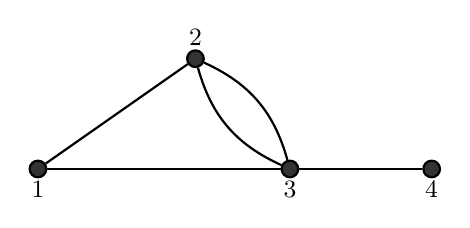
\begin{tikzpicture}[
			every node/.style={circle, draw, fill=black!80, inner sep=0pt, minimum size=6pt},
			lbl/.style={draw=none, fill=none, font=\small},
			thick
			]
			\node[label={[lbl]below:$1$}] (v1) at (0,0) {};
			\node[label={[lbl]above:$2$}] (v2) at (2,1.4) {};
			\node[label={[lbl]below:$3$}] (v3) at (3.2,0) {};
			\node[label={[lbl]below:$4$}] (v4) at (5,0) {};
			\draw (v1) -- (v2);
			\draw (v1) -- (v3);
			\draw[bend left=25]  (v2) to (v3);
			\draw[bend right=25] (v2) to (v3);
			\draw (v3) -- (v4);
		\end{tikzpicture}
	\end{center}

	Степени вершин: $d_1=2$, $d_2=3$, $d_3=4$, $d_4=1$. Лапласиан:
	\[
	L_G =
	\begin{pmatrix}
		2 & -1 & -1 &  0 \\
		-1 &  3 & -2 &  0 \\
		-1 & -2 &  4 & -1 \\
		0 &  0 & -1 &  1
	\end{pmatrix}.
	\]
	(Внедиагональный элемент $l_{23}=-2$ — учтено двойное ребро между $2$ и $3$.)
\end{Example}

\subsection{Матричная теорема Кирхгофа}

\begin{Theorem}{Матричная теорема Кирхгофа}{}
	Для любого графа $G$ и любой вершины $i$:
	\[
	\det\!\bigl((L_G)_{ii}\bigr) = \#\{\text{остовных деревьев в } G\},
	\]
	где $(L_G)_{ii}$ — матрица, полученная вычёркиванием $i$-й строки и $i$-го столбца из $L_G$.
\end{Theorem}

\begin{Remark}{}{}
	Замечательно, что ответ не зависит от того, какую вершину $i$ вычёркивают. Для внедиагонального минора также верно:
	$\det\!\bigl((L_G)_{ij}\bigr) = \pm\,\#\{\text{остовных деревьев в } G\}$.
\end{Remark}

\begin{Remark}{}{}
	Если граф $G$ \emph{несвязен} и распадается на две компоненты
	$\{1,\ldots,k\}$ и $\{k{+}1,\ldots,n\}$, то $L_G$ принимает блочно-диагональный вид:
	\[
	L_G =
	\begin{pmatrix}
		L_{G_1} & 0 \\
		0       & L_{G_2}
	\end{pmatrix}.
	\]
	В каждом блоке сумма строк равна нулю, поэтому строки линейно зависимы и
	$\det\!\bigl((L_G)_{ii}\bigr) = 0$ — остовных деревьев нет, что согласуется с теоремой.
\end{Remark}

\begin{Example}{Проверка по формуле}{}
	Для графа из предыдущего примера вычислим $\det\!\bigl((L_G)_{11}\bigr)$ (вычёркиваем строку и столбец вершины $1$):
	\[
	\det
	\begin{pmatrix}
		3 & -2 &  0 \\
		-2 &  4 & -1 \\
		0 & -1 &  1
	\end{pmatrix}
	= 12 - 3 - 4 = 5.
	\]
	Граф действительно имеет ровно $5$ остовных деревьев: $1 + 2 + 2 = 5$.

	\begin{center}
		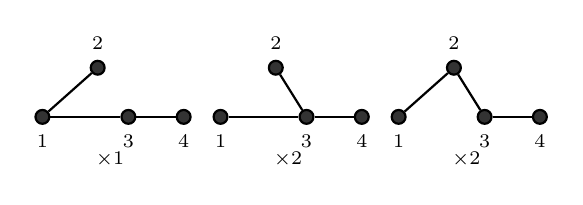
\begin{tikzpicture}[
			scale=0.78,
			v/.style={circle, draw, fill=black!80, inner sep=0pt, minimum size=5pt},
			lbl/.style={font=\scriptsize},
			thick
			]
			% --- дерево 1 (звезда из 3) ---
			\begin{scope}[xshift=0cm]
				\node[v, label={[lbl]below:$1$}] (a1) at (0,0) {};
				\node[v, label={[lbl]above:$2$}] (a2) at (0.9,0.8) {};
				\node[v, label={[lbl]below:$3$}] (a3) at (1.4,0) {};
				\node[v, label={[lbl]below:$4$}] (a4) at (2.3,0) {};
				\draw (a1)--(a2); \draw (a1)--(a3); \draw (a3)--(a4);
				\node[lbl] at (1.1,-0.7) {$\times 1$};
			\end{scope}
			% --- дерево 2a ---
			\begin{scope}[xshift=2.9cm]
				\node[v, label={[lbl]below:$1$}] (b1) at (0,0) {};
				\node[v, label={[lbl]above:$2$}] (b2) at (0.9,0.8) {};
				\node[v, label={[lbl]below:$3$}] (b3) at (1.4,0) {};
				\node[v, label={[lbl]below:$4$}] (b4) at (2.3,0) {};
				\draw (b1)--(b3); \draw (b2)--(b3); \draw (b3)--(b4);
				\node[lbl] at (1.1,-0.7) {$\times 2$};
			\end{scope}
			% --- дерево 3a ---
			\begin{scope}[xshift=5.8cm]
				\node[v, label={[lbl]below:$1$}] (c1) at (0,0) {};
				\node[v, label={[lbl]above:$2$}] (c2) at (0.9,0.8) {};
				\node[v, label={[lbl]below:$3$}] (c3) at (1.4,0) {};
				\node[v, label={[lbl]below:$4$}] (c4) at (2.3,0) {};
				\draw (c1)--(c2); \draw (c2)--(c3); \draw (c3)--(c4);
				\node[lbl] at (1.1,-0.7) {$\times 2$};
			\end{scope}
		\end{tikzpicture}
	\end{center}
	Множители $\times 2$ отвечают за выбор одного из двух параллельных рёбер $\{2,3\}$.
\end{Example}


\begin{figure}[H]
	\centering
	\begin{tikzpicture}[
		v/.style={circle, draw, fill=black!80, inner sep=0pt, minimum size=5pt},
		lbl/.style={font=\small},
		thick, >=Stealth
		]
		% --- G: треугольник, ребро e=12 выделено ---
		\begin{scope}
			\node[v,label={[lbl]left:$1$}]  (g1) at (0,0) {};
			\node[v,label={[lbl]right:$2$}] (g2) at (1.4,0) {};
			\node[v,label={[lbl]above:$3$}] (g3) at (0.7,1.1) {};
			\draw[red, line width=1.2pt] (g1)--(g2) node[midway,below,lbl,black]{$e$};
			\draw (g1)--(g3); \draw (g2)--(g3);
			\node[lbl] at (0.7,-0.9) {$G$};
		\end{scope}
		\node at (2.6,0.4) {\large $\Rightarrow$};
		% --- G-e ---
		\begin{scope}[xshift=3.4cm]
			\node[v,label={[lbl]left:$1$}]  (a1) at (0,0) {};
			\node[v,label={[lbl]right:$2$}] (a2) at (1.4,0) {};
			\node[v,label={[lbl]above:$3$}] (a3) at (0.7,1.1) {};
			\draw (a1)--(a3); \draw (a2)--(a3);
			\node[lbl] at (0.7,-0.9) {$G-e$};
		\end{scope}
		\node at (6.0,0.4) {\large $+$};
		% --- G.e ---
		\begin{scope}[xshift=6.8cm]
			\node[v,label={[lbl]left:$12$}] (b12) at (0,0) {};
			\node[v,label={[lbl]right:$3$}]  (b3) at (1.6,0) {};
			\draw[bend left=32]  (b12) to (b3);
			\draw[bend right=32] (b12) to (b3);
			\node[lbl] at (0.8,-0.9) {$G\cdot e$};
		\end{scope}
	\end{tikzpicture}
	\caption{Рекурсия удаления--стягивания на треугольнике $K_3$ (ребро $e$ выделено). Число остовных деревьев $G$ равно сумме: $G-e$ — путь ($1$ дерево), $G\cdot e$ — две вершины с двойным ребром ($2$ дерева). Итого $3=1+2$ — ровно столько остовных деревьев у $K_3$.}
\end{figure}

\subsubsection*{Доказательство теоремы Кирхгофа}

\begin{proof}
	Доказательство ведётся \textbf{по индукции по числу рёбер} $|E(G)|$.

	\medskip
	\textbf{Лемма (инвариантность относительно нумерации).} \emph{Если переименовать вершины, ответ не меняется}: перестановка вершин одновременно переставляет строки и столбцы $L_G$, что сохраняет нужный минор.

	\medskip
	\textbf{База: $n = 2$, $k$ кратных рёбер.}
	\[
	L_G =
	\begin{pmatrix} k & -k \\ -k & k \end{pmatrix},
	\qquad
	\det\!\bigl((L_G)_{11}\bigr) = k.
	\]
	Это в точности число остовных деревьев: каждое из $k$ рёбер по отдельности соединяет две вершины и даёт отдельное дерево.\checkmark

	\medskip
	\textbf{Переход.} По лемме можно считать, что ребро $e = \{1,2\}$ существует. Используем
	\emph{тождество удаления-стягивания}:
	\[
	\#\,\text{дер}(G) = \#\,\text{дер}(G{-}e) + \#\,\text{дер}(G{\cdot}e),
	\]
	где $G{-}e$ — граф с удалённым ребром $e$, а $G{\cdot}e$ — граф со стянутым ребром $e$.

	Нужно доказать соответствующее тождество для миноров:
	\[
	\det\!\bigl((L_G)_{11}\bigr)
	= \det\!\bigl((L_{G-e})_{11}\bigr) + \det\!\bigl((L_{G\cdot e})_{11}\bigr).
	\]

	Матрицы $L_G$ и $L_{G-e}$ отличаются лишь в $2\times2$-блоке на пересечении первых двух строк и столбцов: $d_2$ заменяется на $d_2{-}1$, а $l_{12}=-(\text{кратность } e)$ заменяется на значение без $e$. Поскольку в миноре $(\cdot)_{11}$ строка и столбец вершины $1$ уже вычеркнуты, отличие сосредоточено в одной диагональной позиции, отвечающей вершине $2$. Разложением по этой строке получаем, что в разность $\det(L_G)_{11} - \det(L_{G-e})_{11}$ вносит вклад только разность диагональных элементов $(d_2) - (d_2{-}1) = 1$:
	\begin{align*}
		\det\!\bigl((L_G)_{11}\bigr) - \det\!\bigl((L_{G-e})_{11}\bigr)
		&= d_2 \cdot M - (d_2{-}1)\cdot M \\
		&= M = \det\!\bigl((L_{G\cdot e})_{11}\bigr),
	\end{align*}
	где $M$ — соответствующий минор, равный определителю минора лапласиана стянутого графа $G\cdot e$. По индукционному предположению (в $G-e$ и $G\cdot e$ рёбер меньше)
	\[
	\det\!\bigl((L_{G-e})_{11}\bigr)=\#\,\text{дер}(G{-}e),\qquad
	\det\!\bigl((L_{G\cdot e})_{11}\bigr)=\#\,\text{дер}(G{\cdot}e),
	\]
	откуда и следует утверждение для $G$.
\end{proof}

\subsection{Деревья в \texorpdfstring{$K_n$}{Kn}. Формула Кэли}

Подсчитаем число остовных деревьев в полном графе $K_n$:

\begin{center}
	\begin{tabular}{c c c}
		\toprule
		$n$ & Число деревьев & $n^{n-2}$ \\
		\midrule
		$1$ & $1$ & $1^{-1} = 1$ \\
		$2$ & $1$ & $2^{0} = 1$ \\
		$3$ & $3$ & $3^{1} = 3$ \\
		$4$ & $16$ & $4^{2} = 16$ \\
		$5$ & $125$ & $5^{3} = 125$ \\
		\bottomrule
	\end{tabular}
\end{center}

Закономерность: число остовных деревьев в $K_n$ равно $n^{n-2}$.

\begin{Remark}{}{}
	Для $n=4$ все $16$ остовных деревьев распадаются на два вида:
	$4$ звезды (одна центральная вершина степени~$3$) и $12$ путей ($4!/2 = 12$).
	Для $n=5$ — три вида: $5$ звёзд, $60$ путей ($5!/2$) и ещё $60$ деревьев с развилкой, итого $5 + 60 + 60 = 125$.

	\begin{center}
		\begin{tikzpicture}[
			v/.style={circle, draw, fill=black!80, inner sep=0pt, minimum size=5pt},
			lbl/.style={font=\scriptsize}, thick, scale=0.85
			]
			% K_3
			\begin{scope}[xshift=0cm, yshift=0cm]
				\node[v] (t1) at (0,0.7) {};
				\node[v] (t2) at (-0.6,0) {};
				\node[v] (t3) at (0.6,0) {};
				\draw (t1)--(t2); \draw (t1)--(t3); \draw (t2)--(t3);
				\node[lbl] at (0,-0.5) {$K_3$, три дерева};
			\end{scope}
			% K_4
			\begin{scope}[xshift=4cm, yshift=0cm]
				\node[v] (q1) at (0,0.8) {};
				\node[v] (q2) at (-0.8,0) {};
				\node[v] (q3) at (0,0) {};
				\node[v] (q4) at (0.8,0) {};
				\draw (q1)--(q2); \draw (q1)--(q3); \draw (q1)--(q4);
				\draw (q2)--(q3); \draw (q2)--(q4); \draw (q3)--(q4);
				\node[lbl] at (0,-0.5) {$K_4$, 16 деревьев};
			\end{scope}
		\end{tikzpicture}
	\end{center}
\end{Remark}

\begin{Theorem}{Формула Кэли}{}
	В полном графе $K_n$ ровно $n^{n-2}$ остовных деревьев.
\end{Theorem}

\begin{proof}
	По теореме Кирхгофа достаточно вычислить $\det\!\bigl((L_{K_n})_{11}\bigr)$.

	Лапласиан $K_n$ имеет вид: на диагонали стоят $n{-}1$, вне диагонали $-1$. Минор
	$(L_{K_n})_{11}$ — матрица $(n{-}1)\times(n{-}1)$:
	\[
	M = \begin{pmatrix}
		n{-}1 & -1 & \cdots & -1 \\
		-1 & n{-}1 & \cdots & -1 \\
		\vdots & & \ddots & \vdots \\
		-1 & -1 & \cdots & n{-}1
	\end{pmatrix}.
	\]

	\textbf{Шаг 1.} Вычтем строку~$1$ из каждой строки $2, \ldots, n{-}1$. Строка $k$ ($k \ge 2$) принимает вид с $-n$ в первой позиции и $n$ в $k$-й:
	\[
	\det M = \det
	\begin{pmatrix}
		n{-}1 & -1 & \cdots & -1 \\
		-n & n & & 0 \\
		\vdots & & \ddots & \\
		-n & 0 & & n
	\end{pmatrix}.
	\]

	\textbf{Шаг 2.} Выносим $n$ из каждой из строк $2, \ldots, n{-}1$ (всего $n{-}2$ строки):
	\[
	\det M = n^{n-2} \cdot \det
	\begin{pmatrix}
		n{-}1 & -1 & \cdots & -1 \\
		-1 & 1 & & 0 \\
		\vdots & & \ddots & \\
		-1 & 0 & & 1
	\end{pmatrix}.
	\]

	\textbf{Шаг 3.} Прибавим к строке~$1$ все строки $2, \ldots, n{-}1$. Первая строка превращается в $(1, 0, \ldots, 0)$, и определитель полученной нижнетреугольной матрицы равен~$1$:
	\[
	\det M = n^{n-2} \cdot \det
	\begin{pmatrix}
		1 & 0 & \cdots & 0 \\
		-1 & 1 & & 0 \\
		\vdots & & \ddots & \\
		-1 & 0 & & 1
	\end{pmatrix}
	= n^{n-2} \cdot 1 = n^{n-2}.
	\]
	Таким образом, число остовных деревьев $K_n$ равно $n^{n-2}$.
\end{proof}
